\subsection{Bedienung}
Die Bedienung wurde für eine übersichtliche und schnelle Anwendung einfach gehalten. Auf der Vorderseite hat es drei Tasten und ein vierzeiliges LCD-Display mit je 16 Charakter für die visuelle Darstellung. Die Tasten sind jeweils aktiv High am Mikrocontroller angeschlossen mittels einem Taster-Pull-Up-Schaltkreis, zu sehen in Abbildung \ref{fig:SwitchPullUp_Software}. Der Pull-Up Widerstand hat einen Wert von $10k\Omega$, der mit einem Taster auf Erde verbunden wird.

\begin{figure}[h]
	\centering
		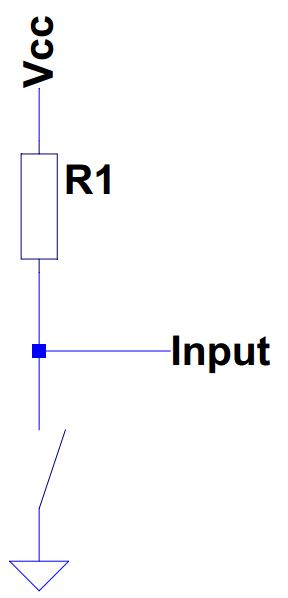
\includegraphics[width=0.15\textwidth]{Taster.jpg}
	\caption{Taster-Pull-Up-Schaltkreis}
	\label{fig:SwitchPullUp_Software}
\end{figure}

Die Taster wurden mit einer Softwarelösung entprellt, ansonsten konnte keine genaue Einstellung der Bestrahlungsstärke erreicht werden, da die Feder im Taster beim Drücken ein undeutliches Signal erzeugt und so ein exaktes und regelmässiges Zählen unmöglich macht. Wird ein Taster betätigt, wird der Widerstand und der Pin des Mikrokontrollers auf Masse verbunden und am Mikrokontroller entsteht ein Low-Zustand, also eine logische Null. Der Tasterzustand wird dann mit der Software ausgelesen.

Das Display stammt von Midas und ist die visuelle Schnittstelle zum Benutzer. Das LCD ist im vier Bit Modus an den Mikrocontroller angeschlossen. Die restlichen Kontakte und der Lesen-Schreiben-Anschluss (Read-Write-Pin) wurden auf Erde verbunden. Der LCD wird mit 5 Volt über den eingebauten DC-DC-Wandler versorgt. Das genaue Anschlussschema  ist in Abbildung \ref{fig:AnschlussSchema} ersichtlich. \todo{Grafik nicht aktuell!}

\begin{figure}[h]
	\centering
		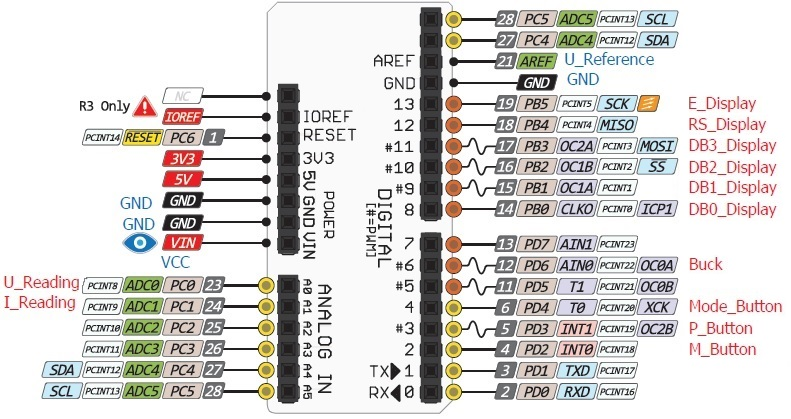
\includegraphics[width=0.8\textwidth]{Anschlussschema.jpg}
	\caption{Anschlussschema für LCD und Tasten am Arduino UNO}
	\label{fig:AnschlussSchema}
\end{figure}